\pdfinfoomitdate=1
\pdftrailerid{}
\documentclass[tikz,border=2pt]{standalone}
\usepackage{newtxtext}
\usepackage{newtxmath}
\definecolor{kafapurple}{RGB}{117,72,141}
\definecolor{kafablue}{RGB}{38,92,140}
\definecolor{kafagreen}{RGB}{55,126,92}
\definecolor{kafateal}{RGB}{30,132,137}
\definecolor{kafaorange}{RGB}{221,132,43}
\definecolor{kafagray}{RGB}{166,166,166}
\begin{document}
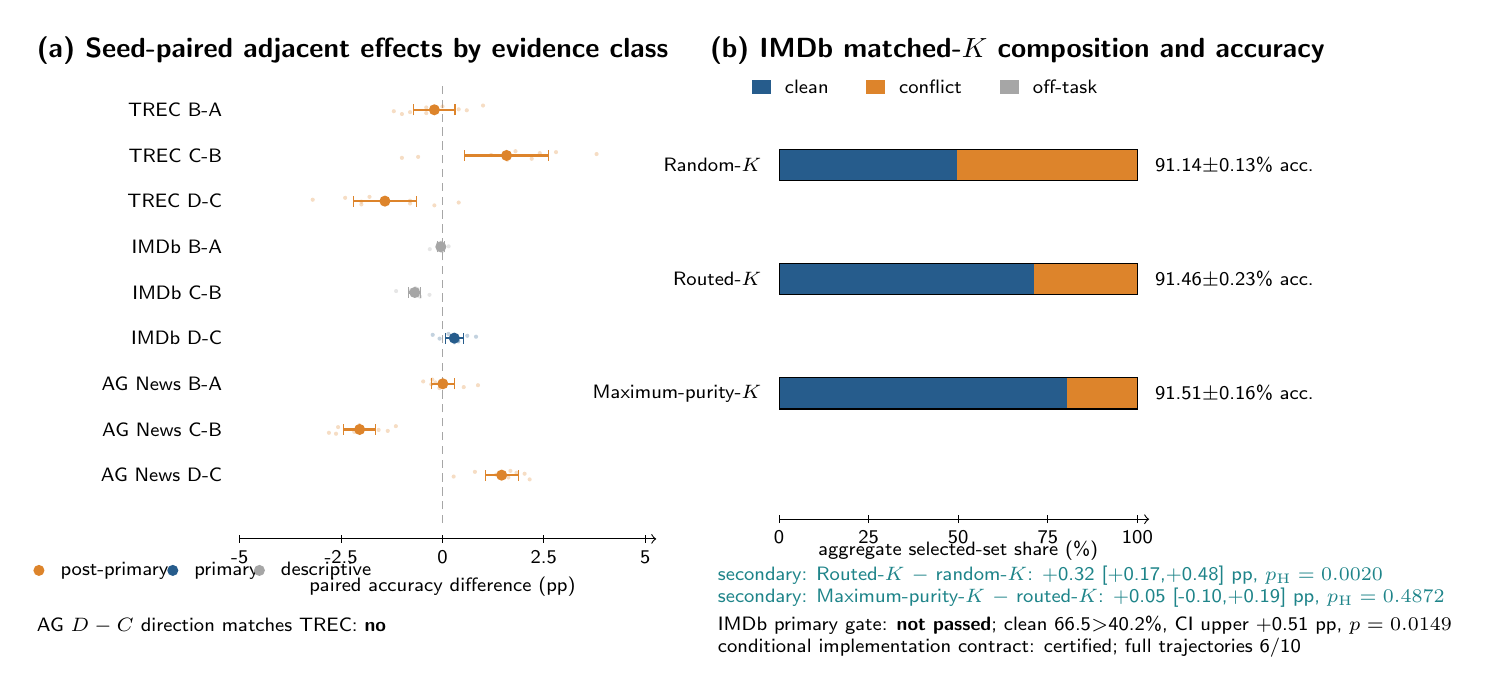
\begin{tikzpicture}[font=\sffamily\scriptsize]
\node[anchor=west,font=\sffamily\bfseries] at (0,7.10) {(a) Seed-paired adjacent effects by evidence class};
\draw[densely dashed,kafagray] (5.275,1.10)--(5.275,6.65);
\fill[kafaorange,opacity=.28] (4.760,6.296) circle (0.75pt);
\fill[kafaorange,opacity=.28] (5.069,6.308) circle (0.75pt);
\fill[kafaorange,opacity=.28] (4.863,6.320) circle (0.75pt);
\fill[kafaorange,opacity=.28] (4.657,6.332) circle (0.75pt);
\fill[kafaorange,opacity=.28] (5.584,6.344) circle (0.75pt);
\fill[kafaorange,opacity=.28] (5.481,6.356) circle (0.75pt);
\fill[kafaorange,opacity=.28] (5.172,6.368) circle (0.75pt);
\fill[kafaorange,opacity=.28] (5.069,6.380) circle (0.75pt);
\fill[kafaorange,opacity=.28] (5.275,6.392) circle (0.75pt);
\fill[kafaorange,opacity=.28] (5.790,6.404) circle (0.75pt);
\node[anchor=east] at (2.600,6.350) {TREC B-A};
\draw[line width=.85pt,kafaorange] (4.910,6.350)--(5.434,6.350);
\draw[kafaorange] (4.910,6.280)--(4.910,6.420) (5.434,6.280)--(5.434,6.420);
\fill[kafaorange] (5.172,6.350) circle (2pt);
\fill[kafaorange,opacity=.28] (6.099,5.716) circle (0.75pt);
\fill[kafaorange,opacity=.28] (6.408,5.728) circle (0.75pt);
\fill[kafaorange,opacity=.28] (4.760,5.740) circle (0.75pt);
\fill[kafaorange,opacity=.28] (4.966,5.752) circle (0.75pt);
\fill[kafaorange,opacity=.28] (6.099,5.764) circle (0.75pt);
\fill[kafaorange,opacity=.28] (5.893,5.776) circle (0.75pt);
\fill[kafaorange,opacity=.28] (7.232,5.788) circle (0.75pt);
\fill[kafaorange,opacity=.28] (6.511,5.800) circle (0.75pt);
\fill[kafaorange,opacity=.28] (6.717,5.812) circle (0.75pt);
\fill[kafaorange,opacity=.28] (6.202,5.824) circle (0.75pt);
\node[anchor=east] at (2.600,5.770) {TREC C-B};
\draw[line width=.85pt,kafaorange] (5.552,5.770)--(6.625,5.770);
\draw[kafaorange] (5.552,5.700)--(5.552,5.840) (6.625,5.700)--(6.625,5.840);
\fill[kafaorange] (6.089,5.770) circle (2pt);
\fill[kafaorange,opacity=.28] (5.172,5.136) circle (0.75pt);
\fill[kafaorange,opacity=.28] (4.245,5.148) circle (0.75pt);
\fill[kafaorange,opacity=.28] (4.863,5.160) circle (0.75pt);
\fill[kafaorange,opacity=.28] (5.481,5.172) circle (0.75pt);
\fill[kafaorange,opacity=.28] (4.245,5.184) circle (0.75pt);
\fill[kafaorange,opacity=.28] (4.863,5.196) circle (0.75pt);
\fill[kafaorange,opacity=.28] (3.627,5.208) circle (0.75pt);
\fill[kafaorange,opacity=.28] (4.554,5.220) circle (0.75pt);
\fill[kafaorange,opacity=.28] (4.039,5.232) circle (0.75pt);
\fill[kafaorange,opacity=.28] (4.348,5.244) circle (0.75pt);
\node[anchor=east] at (2.600,5.190) {TREC D-C};
\draw[line width=.85pt,kafaorange] (4.145,5.190)--(4.942,5.190);
\draw[kafaorange] (4.145,5.120)--(4.145,5.260) (4.942,5.120)--(4.942,5.260);
\fill[kafaorange] (4.544,5.190) circle (2pt);
\fill[kafagray,opacity=.28] (5.273,4.556) circle (0.75pt);
\fill[kafagray,opacity=.28] (5.234,4.568) circle (0.75pt);
\fill[kafagray,opacity=.28] (5.114,4.580) circle (0.75pt);
\fill[kafagray,opacity=.28] (5.267,4.592) circle (0.75pt);
\fill[kafagray,opacity=.28] (5.279,4.604) circle (0.75pt);
\fill[kafagray,opacity=.28] (5.353,4.616) circle (0.75pt);
\fill[kafagray,opacity=.28] (5.275,4.628) circle (0.75pt);
\fill[kafagray,opacity=.28] (5.261,4.640) circle (0.75pt);
\fill[kafagray,opacity=.28] (5.221,4.652) circle (0.75pt);
\fill[kafagray,opacity=.28] (5.261,4.664) circle (0.75pt);
\node[anchor=east] at (2.600,4.610) {IMDb B-A};
\draw[line width=.85pt,kafagray] (5.211,4.610)--(5.297,4.610);
\draw[kafagray] (5.211,4.540)--(5.211,4.680) (5.297,4.540)--(5.297,4.680);
\fill[kafagray] (5.254,4.610) circle (2pt);
\fill[kafagray,opacity=.28] (4.991,3.976) circle (0.75pt);
\fill[kafagray,opacity=.28] (4.954,3.988) circle (0.75pt);
\fill[kafagray,opacity=.28] (5.110,4.000) circle (0.75pt);
\fill[kafagray,opacity=.28] (4.966,4.012) circle (0.75pt);
\fill[kafagray,opacity=.28] (4.884,4.024) circle (0.75pt);
\fill[kafagray,opacity=.28] (4.865,4.036) circle (0.75pt);
\fill[kafagray,opacity=.28] (4.686,4.048) circle (0.75pt);
\fill[kafagray,opacity=.28] (4.877,4.060) circle (0.75pt);
\fill[kafagray,opacity=.28] (4.960,4.072) circle (0.75pt);
\fill[kafagray,opacity=.28] (4.933,4.084) circle (0.75pt);
\node[anchor=east] at (2.600,4.030) {IMDb C-B};
\draw[line width=.85pt,kafagray] (4.844,4.030)--(5.001,4.030);
\draw[kafagray] (4.844,3.960)--(4.844,4.100) (5.001,3.960)--(5.001,4.100);
\fill[kafagray] (4.923,4.030) circle (2pt);
\fill[kafablue,opacity=.28] (5.427,3.396) circle (0.75pt);
\fill[kafablue,opacity=.28] (5.477,3.408) circle (0.75pt);
\fill[kafablue,opacity=.28] (5.471,3.420) circle (0.75pt);
\fill[kafablue,opacity=.28] (5.407,3.432) circle (0.75pt);
\fill[kafablue,opacity=.28] (5.238,3.444) circle (0.75pt);
\fill[kafablue,opacity=.28] (5.434,3.456) circle (0.75pt);
\fill[kafablue,opacity=.28] (5.701,3.468) circle (0.75pt);
\fill[kafablue,opacity=.28] (5.590,3.480) circle (0.75pt);
\fill[kafablue,opacity=.28] (5.151,3.492) circle (0.75pt);
\fill[kafablue,opacity=.28] (5.351,3.504) circle (0.75pt);
\node[anchor=east] at (2.600,3.450) {IMDb D-C};
\draw[line width=.85pt,kafablue] (5.312,3.450)--(5.538,3.450);
\draw[kafablue] (5.312,3.380)--(5.312,3.520) (5.538,3.380)--(5.538,3.520);
\fill[kafablue] (5.425,3.450) circle (2pt);
\fill[kafaorange,opacity=.28] (5.236,2.816) circle (0.75pt);
\fill[kafaorange,opacity=.28] (5.545,2.828) circle (0.75pt);
\fill[kafaorange,opacity=.28] (5.249,2.840) circle (0.75pt);
\fill[kafaorange,opacity=.28] (5.726,2.852) circle (0.75pt);
\fill[kafaorange,opacity=.28] (5.133,2.864) circle (0.75pt);
\fill[kafaorange,opacity=.28] (5.249,2.876) circle (0.75pt);
\fill[kafaorange,opacity=.28] (5.185,2.888) circle (0.75pt);
\fill[kafaorange,opacity=.28] (5.030,2.900) circle (0.75pt);
\fill[kafaorange,opacity=.28] (5.288,2.912) circle (0.75pt);
\fill[kafaorange,opacity=.28] (5.146,2.924) circle (0.75pt);
\node[anchor=east] at (2.600,2.870) {AG News B-A};
\draw[line width=.85pt,kafaorange] (5.131,2.870)--(5.427,2.870);
\draw[kafaorange] (5.131,2.800)--(5.131,2.940) (5.427,2.800)--(5.427,2.940);
\fill[kafaorange] (5.279,2.870) circle (2pt);
\fill[kafaorange,opacity=.28] (3.923,2.236) circle (0.75pt);
\fill[kafaorange,opacity=.28] (3.833,2.248) circle (0.75pt);
\fill[kafaorange,opacity=.28] (4.155,2.260) circle (0.75pt);
\fill[kafaorange,opacity=.28] (4.580,2.272) circle (0.75pt);
\fill[kafaorange,opacity=.28] (4.464,2.284) circle (0.75pt);
\fill[kafaorange,opacity=.28] (4.232,2.296) circle (0.75pt);
\fill[kafaorange,opacity=.28] (4.193,2.308) circle (0.75pt);
\fill[kafaorange,opacity=.28] (3.949,2.320) circle (0.75pt);
\fill[kafaorange,opacity=.28] (4.683,2.332) circle (0.75pt);
\fill[kafaorange,opacity=.28] (4.219,2.344) circle (0.75pt);
\node[anchor=east] at (2.600,2.290) {AG News C-B};
\draw[line width=.85pt,kafaorange] (4.021,2.290)--(4.425,2.290);
\draw[kafaorange] (4.021,2.220)--(4.021,2.360) (4.425,2.220)--(4.425,2.360);
\fill[kafaorange] (4.223,2.290) circle (2pt);
\fill[kafaorange,opacity=.28] (6.382,1.656) circle (0.75pt);
\fill[kafaorange,opacity=.28] (6.022,1.668) circle (0.75pt);
\fill[kafaorange,opacity=.28] (6.112,1.680) circle (0.75pt);
\fill[kafaorange,opacity=.28] (5.417,1.692) circle (0.75pt);
\fill[kafaorange,opacity=.28] (6.022,1.704) circle (0.75pt);
\fill[kafaorange,opacity=.28] (5.957,1.716) circle (0.75pt);
\fill[kafaorange,opacity=.28] (6.318,1.728) circle (0.75pt);
\fill[kafaorange,opacity=.28] (6.215,1.740) circle (0.75pt);
\fill[kafaorange,opacity=.28] (5.687,1.752) circle (0.75pt);
\fill[kafaorange,opacity=.28] (6.138,1.764) circle (0.75pt);
\node[anchor=east] at (2.600,1.710) {AG News D-C};
\draw[line width=.85pt,kafaorange] (5.819,1.710)--(6.235,1.710);
\draw[kafaorange] (5.819,1.640)--(5.819,1.780) (6.235,1.640)--(6.235,1.780);
\fill[kafaorange] (6.027,1.710) circle (2pt);
\draw[->] (2.700,0.900)--(7.990,0.900);
\draw (2.700,0.850)--(2.700,0.950) node[below=2pt] {-5};
\draw (3.988,0.850)--(3.988,0.950) node[below=2pt] {-2.5};
\draw (5.275,0.850)--(5.275,0.950) node[below=2pt] {0};
\draw (6.562,0.850)--(6.562,0.950) node[below=2pt] {2.5};
\draw (7.850,0.850)--(7.850,0.950) node[below=2pt] {5};
\node at (5.275,0.30) {paired accuracy difference (pp)};
\fill[kafaorange] (0.15,0.50) circle (2pt); \node[anchor=west] at (.30,.50) {post-primary};
\fill[kafablue] (1.85,0.50) circle (2pt); \node[anchor=west] at (2.00,.50) {primary};
\fill[kafagray] (2.95,0.50) circle (2pt); \node[anchor=west] at (3.10,.50) {descriptive};
\node[anchor=west,font=\sffamily\bfseries] at (8.55,7.10) {(b) IMDb matched-$K$ composition and accuracy};
\fill[kafablue] (9.20,6.55) rectangle +(0.25,.18); \node[anchor=west] at (9.50,6.64) {clean};
\fill[kafaorange] (10.65,6.55) rectangle +(0.25,.18); \node[anchor=west] at (10.95,6.64) {conflict};
\fill[kafagray] (12.35,6.55) rectangle +(0.25,.18); \node[anchor=west] at (12.65,6.64) {off-task};
\node[anchor=east] at (9.450,5.650) {Random-$K$};
\fill[kafablue] (9.550,5.450) rectangle (11.810,5.850);
\fill[kafaorange] (11.810,5.450) rectangle (14.100,5.850);
\fill[kafagray] (14.100,5.450) rectangle (14.100,5.850);
\draw (9.550,5.450) rectangle (14.100,5.850);
\node[anchor=west] at (14.200,5.650) {91.14$\pm$0.13\% acc.};
\node[anchor=east] at (9.450,4.200) {Routed-$K$};
\fill[kafablue] (9.550,4.000) rectangle (12.781,4.400);
\fill[kafaorange] (12.781,4.000) rectangle (14.100,4.400);
\fill[kafagray] (14.100,4.000) rectangle (14.100,4.400);
\draw (9.550,4.000) rectangle (14.100,4.400);
\node[anchor=west] at (14.200,4.200) {91.46$\pm$0.23\% acc.};
\node[anchor=east] at (9.450,2.750) {Maximum-purity-$K$};
\fill[kafablue] (9.550,2.550) rectangle (13.211,2.950);
\fill[kafaorange] (13.211,2.550) rectangle (14.100,2.950);
\fill[kafagray] (14.100,2.550) rectangle (14.100,2.950);
\draw (9.550,2.550) rectangle (14.100,2.950);
\node[anchor=west] at (14.200,2.750) {91.51$\pm$0.16\% acc.};
\draw[->] (9.550,1.15)--(14.250,1.15);
\draw (9.550,1.10)--(9.550,1.20) node[below=2pt] {0};
\draw (10.688,1.10)--(10.688,1.20) node[below=2pt] {25};
\draw (11.825,1.10)--(11.825,1.20) node[below=2pt] {50};
\draw (12.963,1.10)--(12.963,1.20) node[below=2pt] {75};
\draw (14.100,1.10)--(14.100,1.20) node[below=2pt] {100};
\node at (11.825,0.75) {aggregate selected-set share (\%)};
\node[anchor=west,text=kafateal] at (8.65,0.43) {secondary: Routed-$K$ $-$ random-$K$: +0.32 [+0.17,+0.48] pp, $p_{\mathrm H}=0.0020$};
\node[anchor=west,text=kafateal] at (8.65,0.15) {secondary: Maximum-purity-$K$ $-$ routed-$K$: +0.05 [-0.10,+0.19] pp, $p_{\mathrm H}=0.4872$};
\node[anchor=west] at (8.65,-0.20) {IMDb primary gate: \textbf{not passed}; clean 66.5$>$40.2\%, CI upper +0.51 pp, $p=0.0149$};
\node[anchor=west] at (8.65,-0.48) {conditional implementation contract: certified; full trajectories 6/10};
\node[anchor=west] at (0,-0.20) {AG $D-C$ direction matches TREC: \textbf{no}};
\end{tikzpicture}
\end{document}
